\subsection{De Acciones, a Instrucciones}

Ahora, tenemos las acciones a realizar para poder adaptar la arquitectura de la aplicación hacia el estado de referencia; sin embargo, estas acciones no contienen la información necesaria para ejecutar ninguno de los procesos necesarios.

Partiendo de esto, se determinó la necesidad de una colección estructuras de datos, que contuvieran las instrucciones a realizar, para cada una de las acciones definidas. Así mismo, esta colección, debería especificarse de manera individual para cada locación de la aplicación con el fin de tener una mejor granularidad y control sobre la manera en la que se realizan las modificaciones en la arquitectura.

En consecuencia, como se observa en la figura \ref{fig:Directives}, se definió una estructura de datos llamada \texttt{Directive}. Esta contiene tres campos adicionales para las estructuras \texttt{AdditionOrder}, \texttt{RestartOrder}, y \texttt{ReconfigureOrder}; que corresponden con las acciones \textit{Addition}, \textit{Restart} y \textit{Reconfigure}, respectivamente.

\begin{figure}[ht]
    \centering
    \caption{UML de la estructura de directivas y ordenes}
    \label{fig:Directives}
    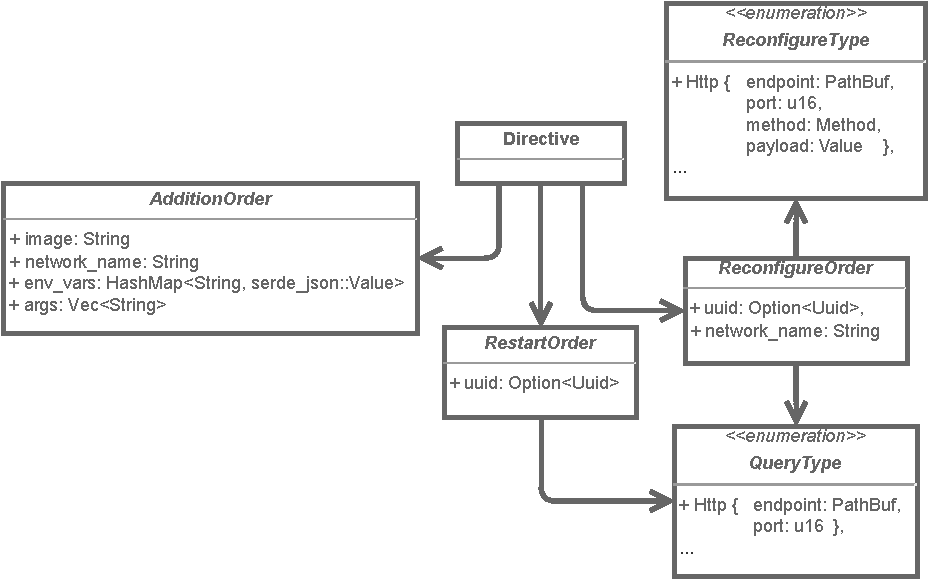
\includegraphics[width=0.8\linewidth]{images/Directives.pdf}
\end{figure}

